% Исходный LaTeX-код (c) Пётр Калинин
% Код распространяется по лицензии GNU GPL (!)

\header{Фундаментальные основы ДП}
\label{fundamental}
Итак, как вы уже, наверное, поняли, общая идея ДП состоит в следующем. Во"=первых, 
\textit{рассмотрим не только ту задачу, ответ на которую надо выводить в выходной файл, но и более 
мелкие, и попробуем в общем случае каждую подзадачу свести к ещё более мелкой}. Во"=вторых, для того, 
чтобы провести это свед\'{е}ние, часто бывает нужно подумать, \textit{чем может оканчиваться} решение 
подзадачи. Это свед\'{е}ние "--- аналог индукционного перехода в матиндукции. Оно в подавляющем 
большинстве случаев выражается в виде некоторого рекуррентного выражения, выражающего ответ на 
подзадачу через ответы на более мелкие подзадачи, но в принципе, конечно, в общем случае чёткое 
выражение не нужно, достаточно \textit{алгоритма} вычисления ответа на подзадачу через ответы на 
мелкие задачи.

При таком сведении естественно получится, что какие"=то, наиболее простые, задачи уже не к чему 
свести "--- их тогда надо решить вручную. Это "--- аналог базы индукции.

В результате легко пишем алгоритм: ответы будем хранить в некотором массиве. Изначально в него 
записываем насчитанные вручную ответы для особых случаев, а потом, обычно в цикле, насчитываем 
остальные ответы.

\lheader{Принцип перекрытия подзадач как причина быстрой работы ДП}
Как же так получается, что ДП работает быстро? Казалось бы, чем ДП лучше перебора, ведь и тот, и 
тот решает много подзадач? Давайте для сравнения напишем переборное решение задачи про черепашку с набором максимальной суммы. 
Перебор пишется легко. 
\begin{codesample}\begin{verbatim}
procedure find(i,j);
begin
if (i=N)and(j=M) then begin
   check;
   exit;
end;
curs:=curs+a[i,j];
if i<N then
   find(i+1,j);
if j<M then
   find(i,j+1);
curs:=curs-a[i,j];
end;






function find(i,j):integer;
var n1,n2:integer;
begin
if i=1 then begin
   if j=1 then
      find:=a[1,1]
   else find:=find(i,j-1)+a[i,j];
   exit;
end;
if (j=1) then begin  {i can't be 1 here}
   find:=find(i-1,j)+a[i,j];
   exit;
end;
n1:=find(i-1,j);
n2:=find(i,j-1);
if n1<n2 then
   find:=n2+a[i,j]
else find:=n1+a[i,j];
end;
\end{verbatim}
\end{codesample}

Тут два варианта написания перебора: в левой колонке "--- полностью в соответствии с тем, как я 
писал в теме про перебор: процедура $find$ перебирает все пути от клетки $(i,j)$ до $(N,M)$; в 
правой колонке "--- немного другой вариант: тут функция перебирает все варианты пути от клетки 
$(1,1)$ до $(i,j)$ и возвращает максимальную возможную сумму (т.е. $find(i,j)$ возвращает то, что 
раньше мы называли $ans[i,j]$). Вдумайтесь в этот вариант, он тоже
довольно простой, и полностью соответствует нашему рекуррентному соотношению, и поэтому намного 
ближе к динамическому решению, поэтому далее я буду иметь ввиду именно его. Тут ещё аккуратно надо 
проверить, учитывается ли начальная клетка в этих решениях; если нет, а надо, или если учитывается, 
а не надо, то исправить легко. В первом варианте в главной программе надо запустить $find(1,1)$, во 
втором "--- $find(N,M)$.

Казалось бы, и ДП, и второй вариант перебора построены на одних и тех же идеях "--- они вычисляют 
решение данной подзадачи через решения более мелких. Но ДП работает намного быстрее. Дело в том, 
что перебор будет по много раз делать одну и ту же работу. Давайте посмотрим работу перебора вглубь 
хотя бы на три шага:

\vspace{0.2cm plus 0.1cm}

\vbox{\footnotesize\obeylines\parindent=0cm\newcommand{\ident}{\raisebox{-2pt}[0pt][0pt]{\rule{0.1pt}{10pt}} \hspace{1cm}}%
Запускается $find(N,M)$ (из главной программы)
\ident Запускается $find(N-1,M)$ (из $find(N,M)$)
\ident \ident Запускается $find(N-2,M)$ (из $find(N-1,M)$)
\ident \ident \ident Запускается $find(N-3,M)$ (из $find(N-2,M)$)
\ident \ident \ident \ident \dots
\ident \ident \ident Запускается $find(N-2,M-1)$ (из $find(N-2,M)$)
\ident \ident \ident \ident \dots
\ident \ident Запускается $find(N-1,M-1)$ (из $find(N-1,M)$)
\ident \ident \ident Запускается $find(N-2,M-1)$ (из $find(N-1,M-1)$)
\ident \ident \ident \ident \dots
\ident \ident \ident Запускается $find(N-1,M-2)$ (из $find(N-1,M-1)$)
\ident \ident \ident \ident \dots
\ident Запускается $find(N,M-1)$ (из $find(N,M)$)
\ident \ident Запускается $find(N-1,M-1)$ (из $find(N,M-1)$)
\ident \ident \ident Запускается $find(N-2,M-1)$ (из $find(N-1,M-1)$)
\ident \ident \ident \ident \dots
\ident \ident \ident Запускается $find(N-1,M-2)$ (из $find(N-1,M-1)$)
\ident \ident \ident \ident \dots
\ident \ident Запускается $find(N,M-2)$ (из $find(N,M-1)$)
\ident \ident \ident Запускается $find(N-1,M-2)$ (из $find(N,M-2)$)
\ident \ident \ident \ident \dots
\ident \ident \ident Запускается $find(N,M-3)$ (из $find(N,M-2)$)
\ident \ident \ident \ident \dots
}

\vspace{0.2cm plus 0.1cm}

Что ж, все ясно. Уже даже здесь видно, что $find(N-1,M-1)$ была запущена \textit{два} раза, и, 
конечно, оба раза честно заново вычисляла максимальную сумму, которую можно набрать по пути от 
$(1,1)$ к $(N-1,M-1)$, хотя совершенно понятно, что сколько раз ни запускай её, ответ всегда будет 
один и тот же. $find(N-2,M-1)$, равно как и $find(N-1,M-2)$ запускалась уже по три раза, и несложно 
догадаться, что чем дальше будет клетка $(i,j)$ от $(N,M)$, тем больше раз будет запускаться 
процедура $find(i,j)$. Эти многократные запуски совершенно бессмысленны, т.к. ответ всегда 
получится один и тот же.

Этим и пользуется динамическое программирование. Вместо того, чтобы каждый раз, когда понадобиться, 
заново считать ответ для $(i,j)$, ДП считает его ровно один раз, а далее просто берет уже известный 
ответ из массива. {\footnotesize На самом деле процедуру $find$ можно написать так, чтобы она 
сначала проверяла, а не запускалась ли она раньше с этими параметрами, и, если, да, то не вычисляла 
ответ заново, а просто возвращала результат, полученный при прошлом запуске и заботливо сохранённый 
в специальном массиве "--- получится то, что называется "<рекурсией с запоминанием результата">, и 
про что я буду говорить ниже.}

Говоря по"=другому, ДП существенно использует тот факт, что ответ на одну и ту же мелкую подзадачу 
будет использоваться далее \textit{несколько} раз, для получения ответов на некоторые более крупные 
подзадачи. Это "--- один из основных принципов ДП, так называемый \textit{принцип перекрытия 
подзадач}. Это именно то, что позволяет ДП работать быстрее "--- намного быстрее "--- перебора.

Рассмотрим дерево перебора для нашего примера переборного решения.

\begin{center}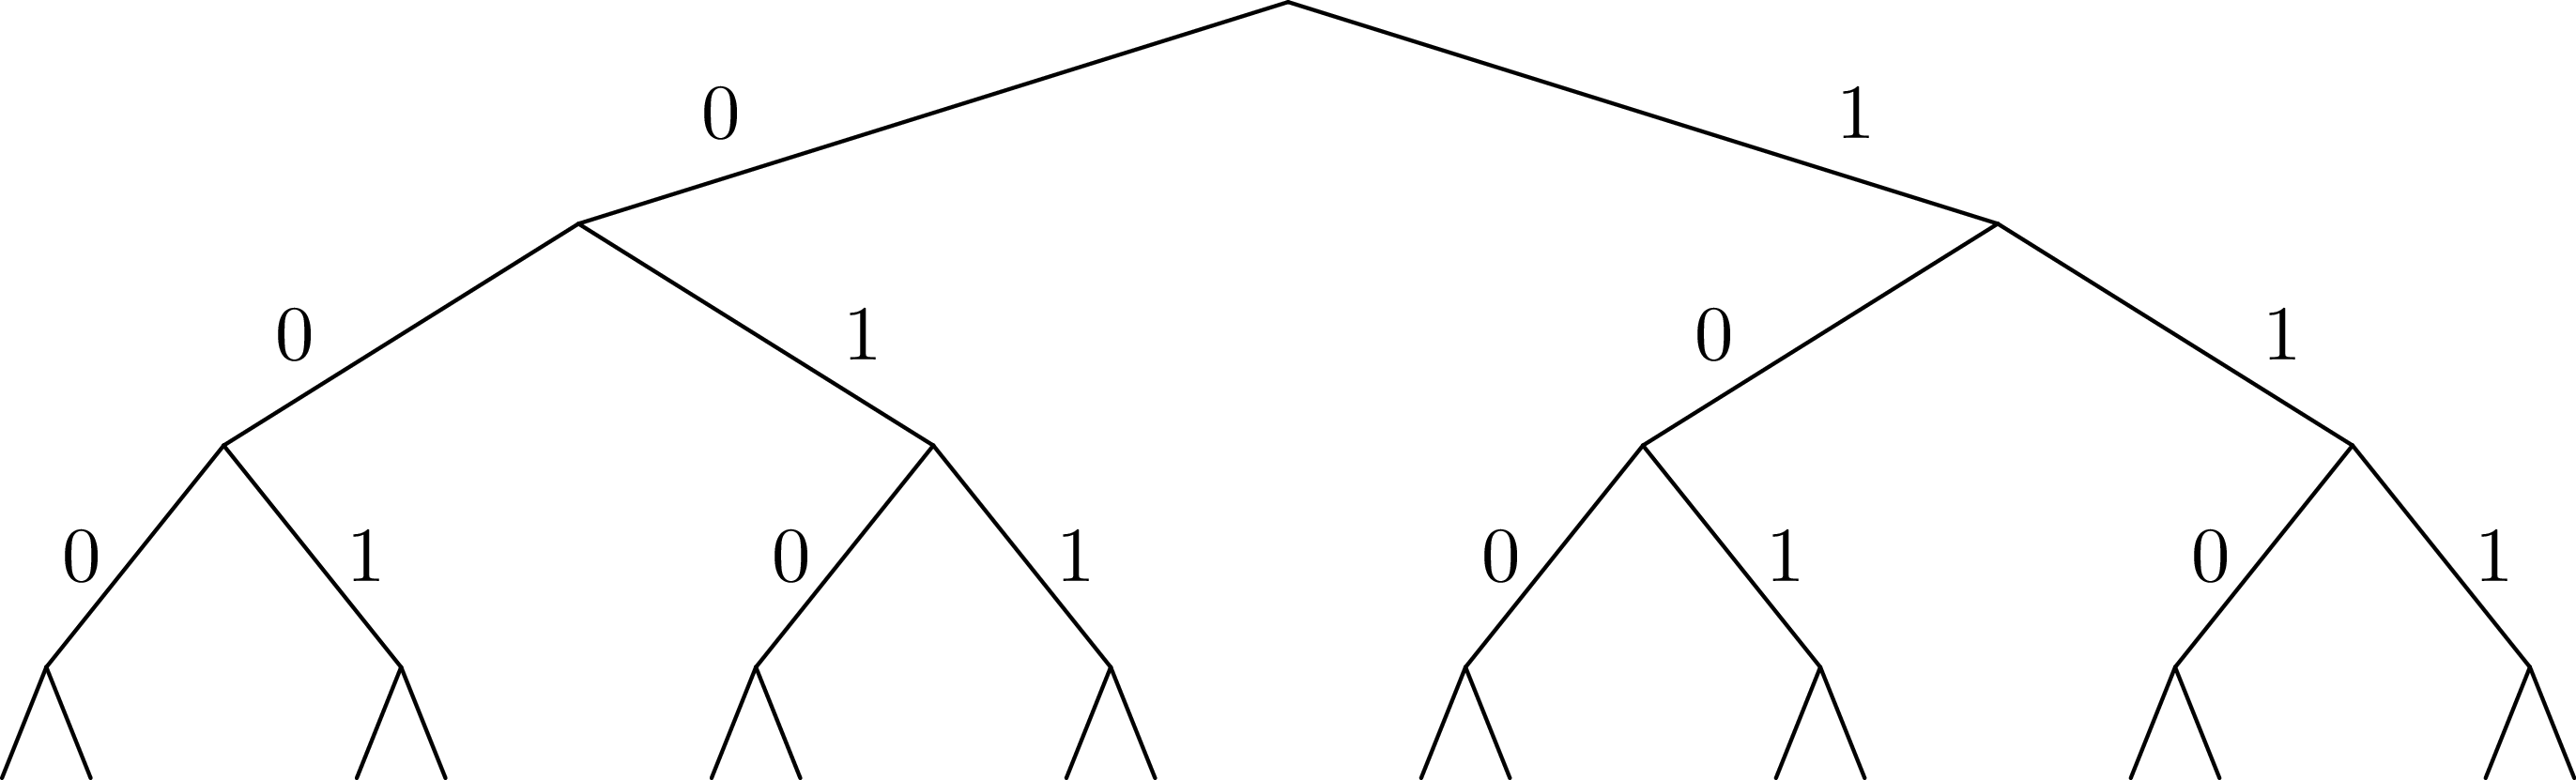
\includegraphics[width=\textwidth]{texts/05_2_fundamental/tree.1}\end{center}

Смысл перекрытия подзадач как раз и состоит в том, что, в частности, выделенные поддеревья 
одинаковы. Поэтому логично их "<объединить">, получая то, что логично называть \textit{графом 
подзадач}:
\begin{center}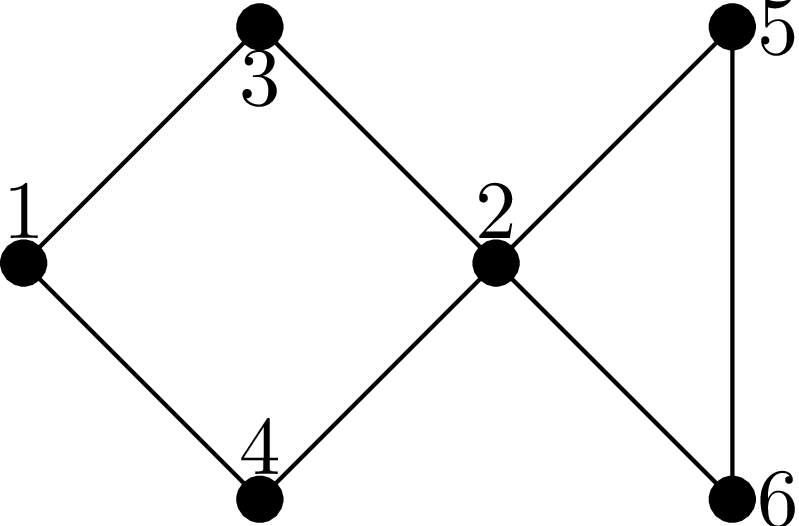
\includegraphics{texts/05_2_fundamental/graph.1}\end{center}

(Естественно, объединяются все экземпляры совпадающих поддеревьев, в частности, все деревья с корнем 
$(N-2,M-1)$ и т.п.)

Представление о графе подзадач будет довольно важно далее. Обратите внимание, что этот граф, конечно же,
ориентированный и ациклический (если бы в нем были бы циклы, то найти все значения было бы не так просто,
а в общем случае и невозможно).

В общем случае вершинами графа подзадач являются все различные подзадачи, которые мы собираемся решать, а
ребра идут от каждой подзадачи $A$ к тем подзадачам, от которых зависит ответ на подзадачу $A$.

\lheader{Принцип оптимальности для подзадач}
Ещё один принцип, который необходим вообще для возможности записи рекуррентного соотношения 
"--- это принцип оптимальности для подзадач. Если вы решаете задачу на оптимизацию (как в задаче про черепашку
с максимизацией суммы), и сводите подзадачу к более мелким, то вам обычно нужно, чтобы решение большой подзадачи 
содержало в себе решения более мелких. Обычно это значит, что любой кусок (или начало, или конец) оптимального решения
подзадачи является оптимальным решением некоторой соответствующей более мелкой подзадачи. Например, в задаче про черепашку
любое начало оптимального пути до любой клетки $(i,j)$ будет оптимальным путём до некоторой другой клетки (т.е. если 
оптимальный путь до клетки $(i,j)$ проходит через клетку $(i',j')$, то соответствующее начало этого пути будет
оптимальным путём до клетки $(i',j')$). 

Если вы сумели придумать, как свести подзадачу к более мелким, это автоматически значит, что принцип оптимальности
для подзадач выполняется, поэтому обычно этот принцип проверяется параллельно с выводом рекуррентного соотношения.

Может показаться, что принцип оптимальности для подзадач выполняется всегда в любых задачах на оптимизацию, но это не так. Он может нарушаться во многих
случаях, например, если в задаче важную роль играет предыстория, например, если набор допустимых на очередном шагу
действий существенно зависит от предыдущих шагов. Пример: пусть в задаче про черепашку черепашке запрещается ходить
в одном и том же направлении более двух раз подряд.

\task|Попробуем, как и раньше, в качестве подзадач рассматривать задачу поиска оптимального пути от $(1,1)$ до $(i,j)$
для всех $i$ и $j$. Поймите, почему принцип оптимальности для подзадач тут не будет выполнен, и, соответственно, почему нельзя
решить эту задачу напрямую аналогично обычной задаче про черепашку.
||||Ну я думаю, задача очевидна. Пусть оптимальный путь $P$ из $(1,1)$ до $(i,j)$ проходит через клетку $(i',j')$. Но из этого вовсе не следует, что соответствующее начало этого пути "--- оптимальный путь до $(i',j')$. Действительно, вполне может быть ещё более хороший путь до $(i',j')$. Раньше, без дополнительного ограничения, мы бы просто заменили начало нашего пути $P$ на этот путь и получили бы ещё более хороший путь до $(i,j)$, а сейчас может не получиться "--- может оказаться, что на стыке более двух раз мы сходили в одну и ту же сторону. Говоря по"=другому: пусть, например, оптимальный путь до $(i',j')$ заканчивается двумя ходами вправо "--- тогда после него мы обязаны будем пойти вверх, а может быть, выгоднее было бы дойти до $(i',j')$ другим, не столь дорогим путём, зато потом иметь право сразу пойти вправо.|

\task|Придумайте, какие подзадачи тут можно рассмотреть, чтобы принцип оптимальности выполнялся, и решите-таки эту 
задачу методом ДП.
||Идея: будем не просто для каждого $i$ и $j$ решать задачу дойти до $(i,j)$, а: для каждого $i$, $j$, $a$ и $b$ (здесь $i$ и $j$ "--- координаты клетки, а $a$ и $b$ каждое может принимать лишь два значения, условно обозначающие ход вверх и вправо) будем искать оптимальный путь до клетки $(i,j)$ среди всех путей, у которых последний ход $b$, а предпоследний "--- $a$ (т.е., например, как оптимальнее всего дойти до $(10,15)$ так, чтобы в конце сходить вправо и потом вверх?) Додумайте, как тут будет производиться свед\'{е}ние к более мелким подзадачам
||Небольшая нетривиальность сведения: в каждой подзадаче $(i,j,a,b)$ мы теперь точно знаем последний ход, и потому точно знаем, откуда мы пришли в клетку $(i,j)$ "--- пусть это клетка $(i',j')$ (её координаты легко вычисляются по $(i,j)$ и $b$). Тогда наша подзадача сводится к одной или двум подзадачам "--- $ans[i',j',c,b]$ с одним или двумя вариантами $c$. Додумайте и обратите внимание, как тут учитывается требование не ходить более двух раз подряд в одну сторону.

Ещё в этой задаче небольшая техническая нетривиальность "--- инициализация начальных значений (на клетках, где нет предпоследнего хода) и обработка первых строк/столбцов. Можете подумать над этим. Тут особенно удобно применить идею нулевых строк и столбцов, о чем я напишу ниже в основном тексте.|

Этот пример показывает, что, если принцип оптимальности для подзадач не выполняется, то иногда это просто обозначает,
что подзадачи плохо выбраны. На самом деле, когда вы выводите рекуррентное соотношение, вы сразу будете видеть,
к каким именно подзадачам сводится данная задача. Может оказаться, что это немного не те подзадачи,
которые вы ожидали "--- значит, надо расширять набор подзадач, которые вы решаете, или как"=то по"=другому
их выбирать.

Но может так быть, что не получается выбрать подзадачи подходящим образом. Например, пусть опять черепашке надо попасть
из $(1,1)$ в $(N,M)$, собрав по дороге максимальную сумму, но при этом заранее известны $K$ векторов, которыми
черепашка может воспользоваться "--- т.е. за один ход черепашка может сдвинуться на любой из этих векторов.
Если каждый вектор $(x,y)$ удовлетворяет одновременно трём условиям $x\geq 0$, $y\geq 0$ и $(x,y)\neq (0,0)$,
то задача не очень сложно решается динамикой за $O(NMK)$ (%
\task|Решите эту задачу||
Решается в точности аналогично простой задаче про черепашку.
||Для каждого $(i,j)$ определим максимальную сумму, которую можно собрать по пути до $(i,j)$. Переберём, какой вектор будет последним ходом, и сравним ответы на соответствующие клетки.
|%
; 
\task|Зачем нужны эти три условия?||
Если ответ ещё не очевиден, то попробуйте посмотреть на ответ на предыдущую задачу и понять, что тут будет не так, если условия не выполняются. Попробуйте представить себе, какой будет граф подзадач, если эти условия не выполняются.
||На самом деле эти условия нужны для того, чтобы граф подзадач был ациклическим. Если эти условия не выполняются, то в общем случае черепашка сможет ходить по циклам, и оптимальный путь так просто динамикой искаться не будет (хотя алгоритмы решения существуют и для такого случая, и даже основанные на идеях ДП, но это уже скорее тематика теории графов, а не ДП). Конечно, может быть так, что граф подзадач будет ациклическим, даже если эти условия не выполняются (попробуйте придумать пример? :) ), и тогда ДП будет работать, только придётся писать рекурсию с запоминанием результата, см. ниже в основном тексте. Но для простоты можно поставить эти условия, чтобы гарантировать ацикличность.
|%
), 
но, если поставить дополнительное условие, что
каждым вектором можно пользоваться не более одного раза, то простой динамикой задача решаться не будет 
(в принципе, тут подойдёт "<динамика по подмножествам">, про которую я буду говорить ниже, но сложность
решения уже не будет полиномиальной, а будет расти как что"=нибудь типа $NMK2^K$).

\task|Поймите, почему тут не работает принцип оптимальности, почему эта задача не решается тупой динамикой и как одно связано с другим.
||||Ну, я думаю, понятно. Как и в прошлом примере, когда черепашке нельзя ходить несколько раз в одну и ту же сторону, тут тоже возникнут проблемы при замене начала пути на соответствующий оптимальный путь: может оказаться, что какой"=то вектор мы используем дважды. Потому не работает принцип оптимальности и потому не работает динамика.

Конечно, можно в подзадачу включить множество векторов, которые мы уже использовали, т.е. "<для каждого $i$, $j$ и набора векторов $M$ найдём оптимальный путь до $(i,j)$, использующий только вектора из множества $M$">. Это и будет динамика по подмножествам. Поскольку всех вариантов для $M$ у нас будет $2^K$, то и сложность будет экспоненциальная.
|

\task|Вспомните задачу про монеты. Там тоже каждой монетой можно было пользоваться не более одного раза,
но при этом задача благополучно решалась динамикой. Чем таким наша задача отличается от задачи про монеты?
Можете ли придумать какую"=нибудь задачу, которая казалась бы близкой к нашей задаче про черепашку, но решалась
бы динамикой аналогично задаче про монеты?
||Может быть, ответ вам сразу очевиден. Может быть, наоборот, вопрос обескураживает. В последнем случае попробуйте перенести идею решения с задачи про монеты на задачу про черепашку и подумайте, что тут не так.
||Отличие между задачами состоит в следующем. В задаче про монеты порядок монет в решении был не важен: если поменять порядок монет в решении, то решение останется решением. А в задаче про черепашку порядок, очевидно, важен: если поменять порядок ходов, то мы посетим совсем другие клетки и потому набранная сумма будет другой. Поэтому в задаче про монеты мы  сумели построить динамическое решение, неявно зафиксировав, в каком порядке берём монеты, а в задаче про черепашку такой фокус не пройдёт.

Соответственно, если в нашей текущей задаче про черепашку интересоваться не максимальной суммой, а вообще вопросом, можно ли дойти до правого верхнего угла с использованием только данных векторов, каждого не более раза, то порядок векторов в ответе будет не важен и эта задача решится динамикой за $O(NMK)$ с ходу без проблем.
|

В общем, оптимальность для подзадач "--- это важный принцип, который выполняется во всех задачах на оптимизацию,
решаемых динамикой, но обычно его специально не проверяют "--- его проверка фактически есть часть доказательства 
рекуррентного соотношения.

\lheader{Дополнительные замечания}
\llheader Введение нулевых элементов. 

\epigraph{Это не физическая величина, а математическое удобство.}{}\nopagebreak

Нередко бывает полезно расширить массив $ans$, введя в нем дополнительные элементы, для того, чтобы особых случаев стало меньше и чтобы б\'{о}льшее количество подзадач решались общим рекуррентным соотношением.

Например, рассмотрим задачу про черепашку с подсчётом количества путей. Раньше у нас были особые случаи $i=1$ или $j=1$. А сделаем следующую идею: введём в массиве $ans$ нулевую строку и нулевой столбец, причём, естественно, $ans[i,0]=ans[0,i]=0$, т.к. до тех клеток невозможно добраться (т.е. есть ноль способов добраться :) ). Теперь несложно видеть, что значения $ans[i,j]$ верно вычисляются по стандартной формуле $ans[i,j]=ans[i-1,j]+ans[i,j-1]$ для всех $i$ и $j$ от 1 до $N$ (или $M$), кроме $ans[1,1]$, который по этой формуле получается ноль, а не один. Можно оставить $ans[1,1]$ особым случаем, но проще сделать, например, $ans[1,0]=1$, и тогда все будет совсем легко.

Аналогично для пути с максимальной суммой можно ввести нулевые строку и столбец и заполнить их значениями $-\infty$ (т.е. меньшими, чем любой возможный ответ на задачу), а элемент $ans[1,0]$ положить равным 0 (или $ans[0,1]$, не важно). Получим:
\begin{codesample}\begin{verbatim}
fillchar(ans,sizeof(ans),0);
ans[1,0]:=1;
for i:=1 to n do
    for j:=1 to m do
        ans[i,j]:=ans[i-1,j]+ans[i,j-1];
заполнить массив ans значениями -inf
ans[1,0]:=0;
for i:=1 to n do
    for j:=1 to m do
        ans[i,j]:=min(ans[i-1,j],ans[i,j-1])+a[i,j];
\end{verbatim}
\end{codesample}
 Обратите внимание, что, если бы мы оставили $ans[1,1]$ особым случаем, то пришлось бы в цикл добавить \verb'if (i<>1)or(j<>1)', что было бы не очень приятно. Ещё обратите внимание, что для удобства я весь массив инициализирую нулями (или минус бесконечностями), хотя достаточно только нулевые элементы.
 
Итак, общая идея введения нулевых элементов: иногда бывает полезно расширить массив $ans$ и
проинициализировать новые элементы так, чтобы все значения в основной части массива можно было
вычислять по общей формуле. Именно это является основным критерием корректности введения нулевых
элементов. В подавляющем большинстве случаев их значения довольно естественны (конечно, ведь
черепашка не может добраться до клетки $(3,0)$ никоим образом "--- поэтому $ans[3,0]=0$), но не
всегда ($ans[1,0]$ тому пример), поэтому проверяйте корректность введения нулевых элементов именно
по тому, что остальные элементы считаются нормально. Поэтому полезно сначала значения определять из
этих естественных соображений, но потом обязательно проверять, что остальные значения считаются
нормально. Ещё раз: единственный критерий правильности определения значений нулевых элементов "--- 
то, что другие элементы считаются правильно, а различные другие качественные соображения "--- 
лишь дополнительная подсказка, хотя нередко и полезная.

\taskn{Контрольный вопрос}|Понимаете ли вы, что остальные элементы в этих примерах считаются корректно?|||||

Достоинство введения нулевых элементов в том, что, во"=первых, частных случаев и, главное, кода для них становится существенно меньше (сравните этот код для черепашки с тем, что был раньше), а во"=вторых в том, что вывод решения станет проще (см. далее).

Название "<нулевые элементы">, конечно, довольно условно "--- они могут в разных задачах быть и 
первыми, и минус первыми, и т.д.

Аналогично нулевые элементы можно ввести и в двух других рассмотренных ранее задачах. В задаче про последовательности из нулей и единиц большого смысла в этом нет, там как ни крути, а два особых случая нужны, но можно ради красоты понять, что $ans[0]=1$ (действительно, тогда $ans[2]$ посчитается правильно "--- и логично, ведь есть только одна строка длины ноль "--- пустая строка), и тогда инициализировать только $ans[1]$ и $ans[0]$, а основной цикл писать от двух. В принципе, это, может быть, потом сыграет при выводе $k$-й по счету последовательности, но пока нам введение нулевого элемента здесь ничего не даёт.

А вот в задаче про монеты очень естественно рассмотреть $i=0$. Не имея ни одной монеты, нельзя набрать ничего, кроме нуля, поэтому $ans[0,0]=true$, а остальные $ans[0,j]=false$ "--- и действительно, несложно проверить, что остальные элементы будут считаться правильно. Поэтому инициализируем нулевую строку массива и дальше основной цикл идёт с единицы, а не с двойки. Это не сильно упрощает алгоритм (будет одно присваивание в особых случаях, а не два), но для задания \ref{multi_coins} про возможность использования одной монеты много раз введение нулевой строки уже поможет сильнее; также далее будет видно, что выводить само решение также проще, если ввести нулевую строку.

\llheader Хранение только последних строк таблицы. Обычно подзадачи, которые мы решаем, характеризуются одним или несколькими
индексами $i$, $j$, \dots{} (хотя бы потому, что ответы надо хранить где"=то в массиве). Нередко бывает так, что один (или
несколько) из этих индексов (пусть $i$) таковы, что все ребра нашего графа подзадач идут между подзадачами, у которых
$i$ отличается ненамного. Т.е. задача с индексами $i$, $j$, \dots{} зависит только от задач с индексами $i'$, $j'$, \dots{}
такими, что $i-q\leq i'\leq i$, где $q$ "--- не очень большое число. Например, в задаче про черепашку $q=1$: задача $(i,j)$
зависит только от задач $(i-1,j)$ и $(i,j-1)$; аналогично в задаче про монеты задача $(i,j)$ зависит только от задач $(i-1,j')$
с некоторыми $j'$. В задаче про 01"=последовательности задача $i$ зависит только от $i-1$ и $i-2$.

Нередко программу решения таких задач можно написать так, что самый внешний цикл будет циклом по тому же индексу $i$ (именно так и 
написаны все примеры выше). В таком случае очевидно, что, если мы уже дошли в этом цикле до $i=100$, 
то нам скорее всего не надо помнить \textit{все} насчитанные ранее значения; достаточно только помнить значения с
$i=100$, $i=99$, \dots, $i=100-q$; остальные нам никогда больше не понадобятся.

Поэтому можно написать программу немного по"=другому. Будем хранить ответы только на подзадачи с текущим $i$, а также на подзадачи
с несколькими предыдущими $i$. Например, если $q=1$ (т.е. задача $i$ связана только с $i-1$), то будем хранить два массива,
$cur$ и $old$ "--- ответы на подзадачи с текущим и предыдущим $i$ соответственно (далее я буду называть множество таких ответом 
\textit{строкой} таблицы, хотя в общем случае, конечно, это может быть и одно число, и одномерный массив, и многомерный массив,
в зависимости от того, сколько ещё индексов характеризует нашу задачу). В цикле будем вычислять все элементы $cur$, используя
$old$ и, при необходимости, уже насчитанные элементы $cur$, а потом сделаем $old:=cur$ и перейдём на следующую итерацию цикла.

Например, в задаче про черепашку с насчетом числа способов:
\begin{codesampleo}\begin{verbatim}
var cur,old:array[0..maxM] of integer;
...
fillchar(old,sizeof(old),0);
old[1]:=1;
for i:=1 to N do begin
    cur[0]:=0;
    for j:=1 to M do
        cur[j]:=cur[j-1]+old[j];
    old:=cur;
end;
\end{verbatim}
\end{codesampleo}
Ответ лежит в $cur[M]$ (и в $old[M]$, конечно). Здесь я уже ввёл нулевые элементы, как писал выше. В цикле всегда
(точнее, до последней строки) $old[j]$ соответствует $ans[i-1,j]$ в предыдущих реализациях, а $cur[j]$ "--- $ans[i,j]$.
По аналогии со сказанным выше, я инициализирую все нулевые элементы нулями, кроме $ans[0,1]$, который теперь есть
$old[1]$ в начале программы (догадайтесь, почему именно $ans[0,1]$, а не $ans[1,0]$ :) ). Надеюсь, что этот пример прояснил
довольно мутные мои рассуждения, написанные выше.

\task|Напишите аналогично задачу про монеты.||||
\begin{codesampleo}\begin{verbatim}
fillchar(old,sizeof(old),false);
old[0]:=true;
for i:=1 to n do begin
    for j:=0 to s do
        if j<a[i] then
           ans[j]:=old[j]
        else ans[j]:=old[j] or old[j-a[i]];
    old:=ans;
end;
\end{verbatim}
\end{codesampleo}
|


В ситуации, когда $q>1$, можно или завести несколько переменных, в которых хранить отдельные строки массива, а в конце цикла
делать что"=нибудь в стиле $a:=b;$ $b:=c;$ $c:=d;$ \dots, либо хранить последние $q+1$ строку (соответствующие
$i$, $i-1$, $i-2$, \dots, $i-q$) в массиве типа \texttt{array[0..q, ...]}. Можете додумать второй вариант сами,
а первый способ продемонстрирую на примере задачи про 01"=последовательности:
\begin{codesampleo}\begin{verbatim}
a:=1;
b:=2;
for i:=2 to n do begin
    c:=a+b;
    a:=b;
    b:=c;
end;
\end{verbatim}
\end{codesampleo}
Здесь $c=ans[i]$, $b=ans[i-1]$, $a=ans[i-2]$.

Зачем все это нужно? В первую очередь для того, чтобы экономить память. Если вы, например, решаете задачу про монеты
с $N=S=10\,000$, то в ограничение времени вы, скорее всего, уложитесь (сложность алгоритма $O(NS)$, и константа невелика),
но вам нужен будет массив порядка $10\,000\times 10\,000$. На Borland Pascal
вам никто столько не даст, да и на Delphi вы, скорее всего, в ограничение по памяти не влезете. 
Если же вы напишите решение с сохранением только последних строк таблицы,
то в память спокойно уложитесь.

Правда, обычно все не так плохо, и на дельфях памяти обычно хватает, поэтому эта идея намного чаще 
используется, если вы пишете на BP. Тем не менее все равно, даже если пишете на дельфи, полезно на всякий случай 
представлять себе, что такое бывает, и быть готовым применить этот приём.

Ещё замечу, что это все не работает, если вам нужно восстанавливать решение, про что речь пойдёт ниже.

И наконец совсем особый случай. Иногда бывает возможно совместить массивы $old$ и $cur$ в одном 
массиве "--- получится код, корректность которого будет не очевидна, но который в принципе может работать. Особенно часто 
это бывает для задач типа набора чего"=нибудь. Например, в задаче про монеты можно написать 
\begin{codesampleo}\begin{verbatim}
fillchar(ans,sizeof(ans),false);
ans[0]:=true;
for i:=1 to n do
    for j:=s downto a[i] do
        ans[j]:=ans[j] or ans[j-a[i]];
\end{verbatim}
\end{codesampleo}

Разберитесь, почему это работает (может быть, полезно вручную промоделировать), и почему цикл по 
$j$ идёт от б\'{о}льших значений к меньшим. Обратите внимание на то, как мы избавились от if'а.
\task|Какую задачу будет решать этот же код, но с циклом по $j$ в обратном порядке, т.е.
от $a[i]$ до $s$?||||Если подумать, то очевидно, что задачу \ref{multi_coins} про монеты с неограниченным количеством монет каждого достоинства.|

Подобный способ написания динамики иногда можно применять, но с осторожностью, т.е. только 
убедившись, что все точно работает. 

Кстати, такому коду, пожалуй, можно даже придумать полноценное ДПшное оправдание. Можете придумать 
:)